\chapter{مقدمه}
\section{بسیار}
\subsection{راحت}

\section{مراجل}
در این فصل به مروری بر مفاهیم بکار رفته در این پایان‌نامه مبادرت می‌ورزیم. پر واضح است که یادگیری این مفاهیم، درک دیگر مفاهیم اشاره شده در فصول دیگر را تسهیل می‌نماید. کار را با بررسی مفاهیم نهان‌سازی آغاز می‌نماییم، سپس در دو بخش مجزا به سراغ مفاهیم و موضوعات مرتبط با نهان‌کاوی و نشان‌گذاری، می‌رویم. 

\section{نهان‌سازی اطلاعات}
\label{InformationHiding}
\index{نهان‌سازی اطلاعات}
\lr{Herodotus} 
در 440 سال قبل از میلاد، به دنبال راهی می‌گشت تا به طور امن بتواند پیغام خود را ارسال کند. مطمئنا ‎ ‎\glspl{Agreed}‎ به تنهایی نمی‌توانست امنیت پیام او را تضمین کند. چراکه کوچکترین شک دشمن مبنی بر ارسال هرگونه پیام محرمانه، موجب  قطع کانال مخابراتی او می‌شد. تراشیدن سربردگان، خال‌کوبی پیام بر روی سرآن‌ها و رشد مجدد موی سر بردگان، به او تضمین می‌داد که بدون هیچ‌گونه شکی از ناحیه دشمن می‌تواند پیام خود را انتقال دهد. کاری که {\lr{Herodotus}} انجام داد.
 
امروزه علم نهان‌سازی اطلاعات، رشد و گسترش زیادی پیدا کرده و به دلیل نوع کاربردهای آن، از اهمیت حیاتی نیز برخوردار گشته است. به عنوان مثال:
\begin{itemize}
\X
مطمئنا هیچ دولتی دوست ندارد، که بسترهای مخابراتیش، به محملی برای مبادله پیام‌های پنهانی، بدون اطلاع آن‌ها تبدیل شود؟!  
\X
شاید تهیه‌کننده فیلم قلب یخی، بسیار علاقه دارد تا به نحوی جلوی جعل و کپی برداری های غیرمجاز از فیلمش را بگیرد، تا به نحوی از ورشکست شدن فرار کند؟
\X
شاید نهان‌سازی تنها راهی باشد که یک سفیر برای مبادله پیام به کشورش باید انتخاب کند؛ چرا که مطمئنا تمام ارتباطاتش به شدت تحت کنترل می‌باشد. 
\end{itemize}
نهان‌سازی اطلاعات، یک واژه عمومی‌است، که تعداد زیادی از مسایل مربوط به درج   ‎\glspl{Aggregate}‎ در یک در برمی‌گیرد. شکل {\ref{InformationHidingHierarch}} بر آن است تا زیرشاخه های علم نهان‌سازی اطلاعات را نشان دهد. 

\begin{figure}
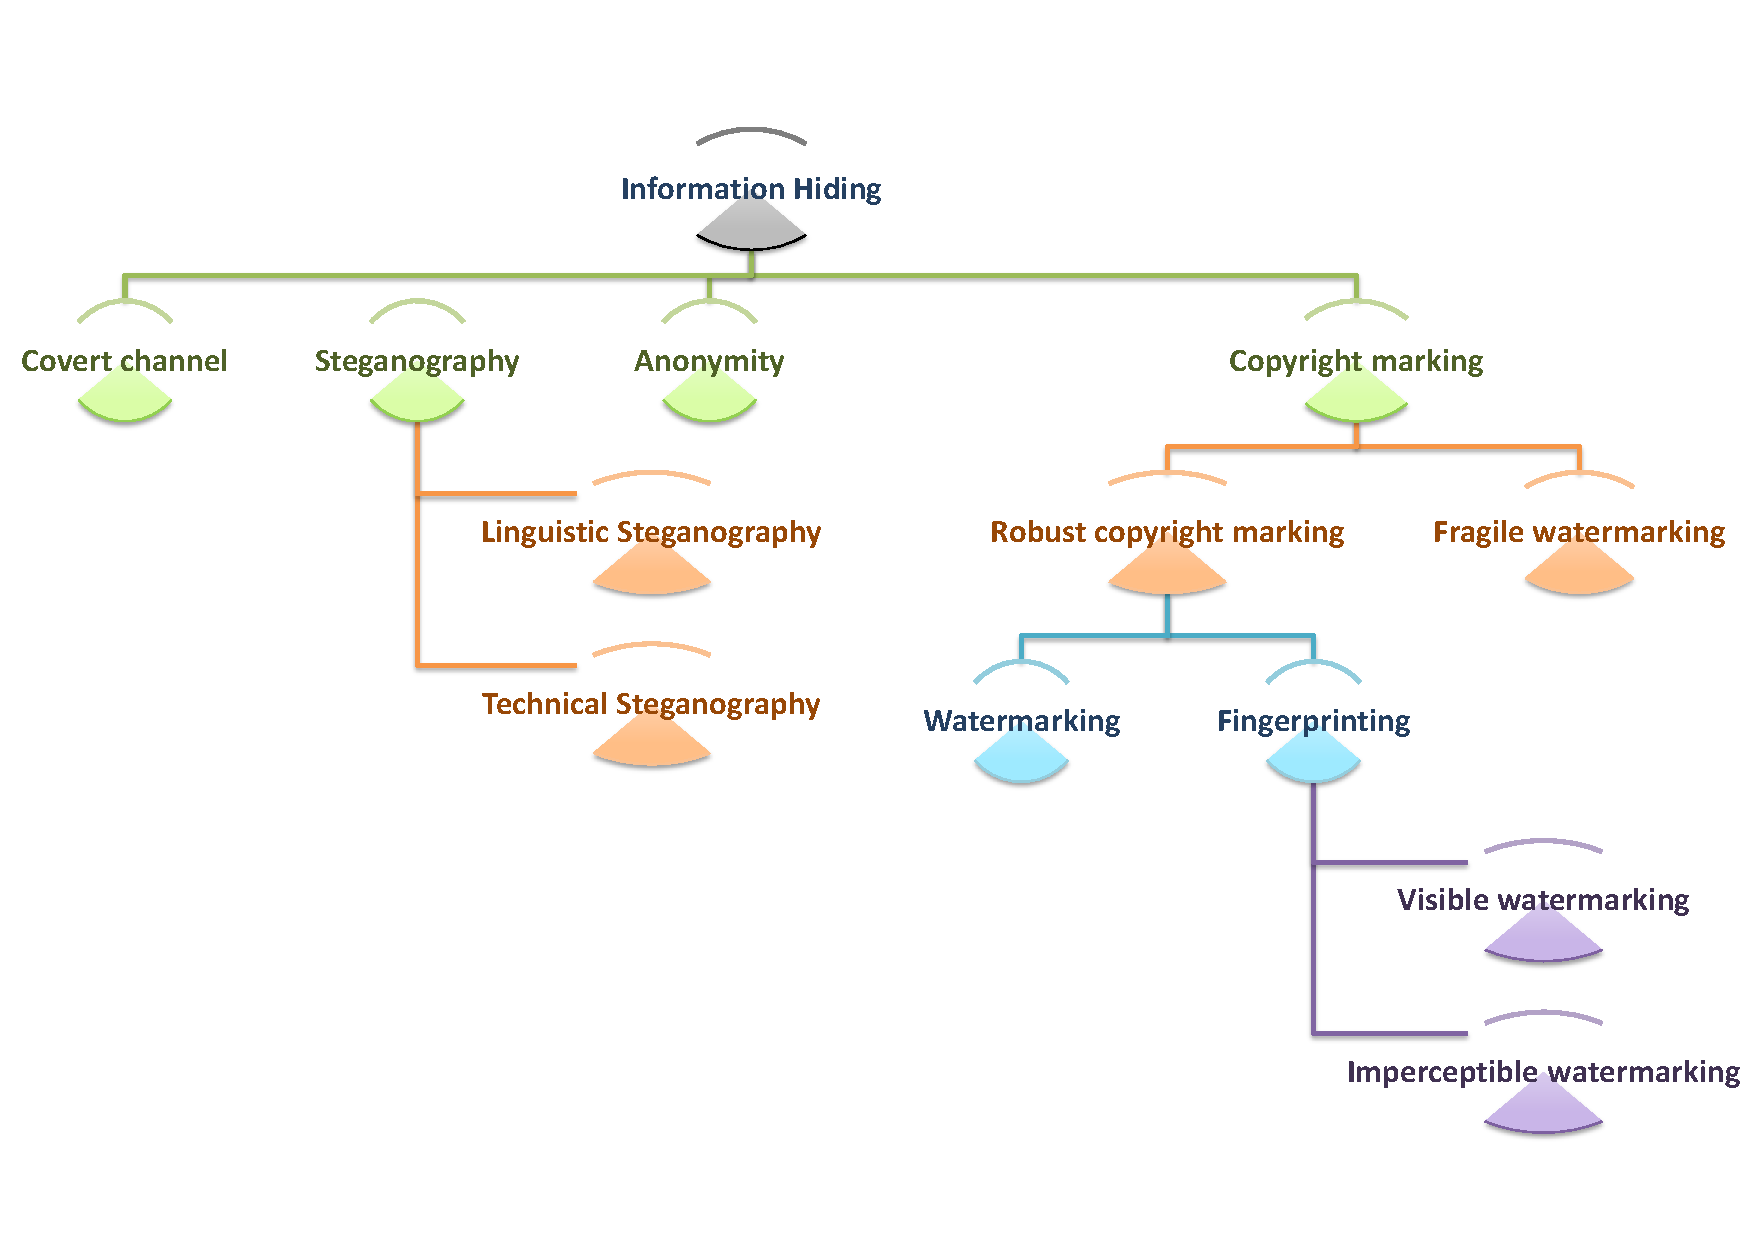
\includegraphics[width=.9\textwidth ,height=.65\textwidth]{Pic/InformationHidingHierarch}
\caption{زیرشاخه‌های علم نهان‌سازی اطلاعات}
\label{InformationHidingHierarch}
\end{figure}

نهان‌سازی به مانند رمزنگاری علمی است چالش برانگیز؛ چراکه در نقطه مقابل نهان‌ساز، فرد یا افرادی وجود دارند، که می‌خواهند کار نهان‌ساز را با شکست مواجه کنند. در این پایان‌نامه ما در دو چهره ظاهر می‌شویم. در چهره اول به عنوان نهان‌ساز به سراغ  می‌رویم، و روشی را در زمینه نشان‌گذاری فایل‌های ویدئویی ارایه می‌دهیم. در چهره بعدی ما دشمن نهان‌ساز می‌شویم. در این چهره به سراغ   ‎\glspl{AggregateFunction}‎  رفته و سعی در کشف پیامی می‌کنیم، که نهان‌نگار آن را در یک سیگنال تصویر پنهان نموده است. 

در نشان‌گذاری به سراغ ویدئو رفتیم؛ چراکه اولا به نظر می‌رسد، نشان‌گذاری در سیگنال تصویر به رشد و بالندگی قابل قبولی رسیده باشد، و الان نیکو است که محور ثقل مطالعات بر روی نشان‌گذاری در ویدئو معطوف شود. دوما به نظر می‌رسد نشان‌گذاری در ویدئو کاربرد بیشتری نسبت به نشان‌گذاری در  تصویر داشته باشد. اما در نهان‌نگاری قضیه کاملا بالعکس است. لذا در مجموع محور مطالعات را بر روی نشان‌گذاری در ویدئو و نهان‌کاوی تصویر، قرار دادیم. 


\section{نهان‌نگاری و نهان‌کاوی}
\label{SteganalysisIntro}

اولین کسی که در تاریخ از این واژه استفاده نمود، فردی به نام {\lr{Johannes Trithemius}} که در سال 1499 در کتابی در مورد جادو، از این واژه استفاده نمود. 

\subsection{آشنایی با چند مفهوم}
برای طی ادامه مسیر لازم است که با برخی مفاهیم موجود در علم ....

\begin{dingautolist}{182}
\item
آیا پیامی‌در سیگنال پنهان شده است یا نه؟
\item
بدست آوردن اطلاعات جانبی از پیام، همچون طول پیامی که پنهان شده است؟
\item
بدست آوردن اصل پیام پنهان شده.
\end{dingautolist}
مهم ترین وظیفه یک نهان‌کاو تشخیص.
\begin{description}
\item[سیگنال پوشش:]\index{سیگنال پوش}
\inpdic{سیگنال پوشش}{Cover Signal}
، سیگنالی است که قصد داریم، در آن پیامی پنهان کنیم. این سیگنال می‌تواند یک تصویر، ویدئو و ... باشد. 
\item[خطای نوع اول:]\index{خطای نوع اول}
خطای نوع اول که آن را با نام {\lr{False Positive}} نیز می‌شناسیم، بدین معنی است که فرستنده پیامی پنهان نکرده باشد، ولی نهان‌کاو به اشتباه بگوید که پیامی در سیگنال پنهان شده است. 
\item[خطای نوع دوم:]\index{خطای نوع دوم}
خطای نوع دوم که آن را با نام {\lr{True Negative}} نیز می‌شناسیم، بدین معنی است که فرستنده پیامی در سیگنال پنهان کرده باشد،
\end{description}


آوردن یک جدول:
\begin{table}
\renewcommand{\arraystretch}{1.35}
\caption{نتایج حمله فشرده سازی \lr{MPEG-4}}
\centering
\begin{tabular}{|c||c|c|c|c|}
\hline
\tablefont{نرخ بیت}&
\tablefont{$1506kbps$}&\tablefont{$1775kbps$}&\tablefont{$1981kbps$}&\tablefont{$2378kbps$}\\\hline
\tablefont{درصد خطا}&\tablefont{$6.05$}&\tablefont{$1.76$}&\tablefont{$0.19$}&\tablefont{$0.58$}\\\hline
\end{tabular}
\label{mpegAttackTable}
\end{table}


\begin{table}
\caption{نتایج حمله بهره}
\centering
\begin{tabular}{|c||c|c|c|c|c|c|}
\hline
\tablefont{ویدئو}&\tablefont{$.1$}&\tablefont{$.3$}&\tablefont{$.5$}&\tablefont{$1.3$}&\tablefont{$1.5$}&\tablefont{$1.7$}\\\hline
\tablefont{foreman}&\tablefont{$0$}&\tablefont{$0$}&\tablefont{$0$}&\tablefont{$2.18$}&\tablefont{$3.24$}&\tablefont{$4.96$}\\\hline
\tablefont{claire}&\tablefont{$3.32$}&\tablefont{$0$}&\tablefont{$0$}&\tablefont{$1.05$}&\tablefont{$0.74$}&\tablefont{$1.32$}\\\hline
\tablefont{hall monitor}&\tablefont{$0$}&\tablefont{$0$}&\tablefont{$0$}&\tablefont{$0$}&\tablefont{$2.03$}&\tablefont{$5.39$}\\\hline
\tablefont{momdaughter}&\tablefont{$0$}&\tablefont{$0$}&\tablefont{$0$}&\tablefont{$0$}&\tablefont{$1.25$}&\tablefont{$2.93$}\\\hline
\end{tabular}
\label{gainAttackTable}
\end{table}

\section{تاثیر تغییر ضریب قدرت }
در این شبیه سازی طول قالب سه بعدی را برابر با $16 \times 16 \times 16$ است. مقدار $\alpha $ را از $1.001$ تا $1.039$ تغییر می‌دهیم. حمله  نویز سفید با انحراف استاندارد 20 را در کانال اعمال می‌کنیم. نتایج برای پنج فایل ویدئویی به صورت زیر است. در این حالت 256 بیت در هر سیگنال پنهان شده است. 











